\lstinputlisting[language=bash,basicstyle=\small]{python_codes/fieldstone_15/keywords.ascii}

\begin{center}
Code at \url{https://github.com/cedrict/fieldstone/tree/master/python_codes/fieldstone_15}
\end{center}

\par\noindent\rule{\textwidth}{0.4pt}
%%%%%%%%%%%%%%%%%%%%%%%%%%%%%%%%%%%%%%%%%%%%%%%%%%%%%%%%%%%%%%%%%%%%%%%%%%%%%%%%%%%%%%%%%%%%

The details of the numerical setup are presented in Section~\ref{mms1}.
The main difference resides in the Schur complement approach to solve the 
Stokes system, as presented in Section \ref{sec:solvers} (see {\bf solver\_cg}).
This iterative solver is very easy to implement once the blocks $\K$ and $\G$, 
as well as the rhs vectors $f$ and $h$ have been built. 

\begin{center}
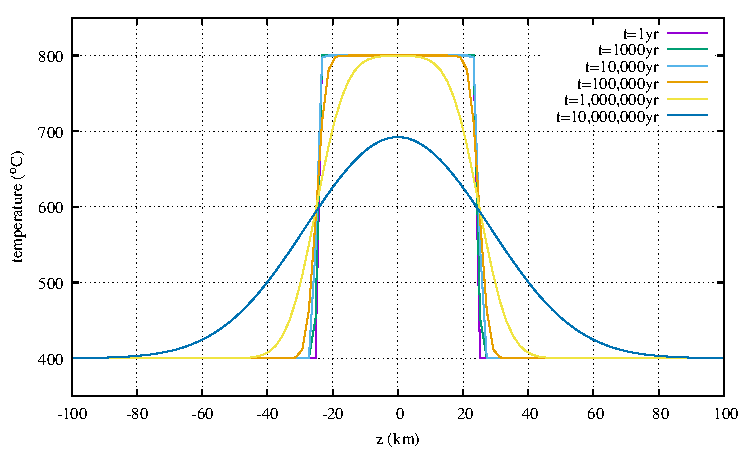
\includegraphics[width=15cm]{python_codes/fieldstone_15/results/solution.pdf}\\
{\captionfont Solution plot automatically generated with matplotlib.}
\end{center}

Rather interestingly the pressure checkerboard modes are not nearly as present as 
in \stone~01 which uses a full matrix approach. 

Looking at the discretisation errors for velocity and pressure, we 
of course recover the same rates and values as in the full matrix case.

\begin{center}
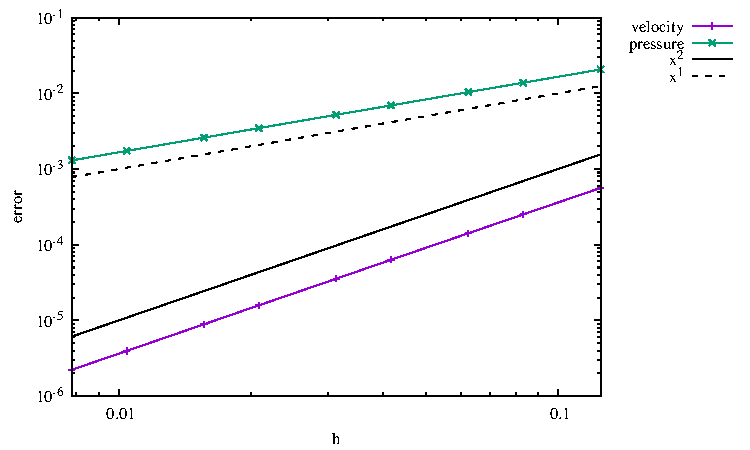
\includegraphics[width=10cm]{python_codes/fieldstone_15/results/errors.pdf}
\end{center}

Finally, for each experiment the normalised residual (see {\bf solver\_cg}) was recorded. We see that 
all things equal the resolution has a strong influence on the number of iterations the solver must
perform to reach the required tolerance. This is one of the manifestations of the fact that the 
$Q_1 \times P_0$ element is not a stable element: the condition number of the matrix increases with 
resolution. We will see that this is not the case of stable elements such as $Q_2\times Q_1$.

\begin{center}
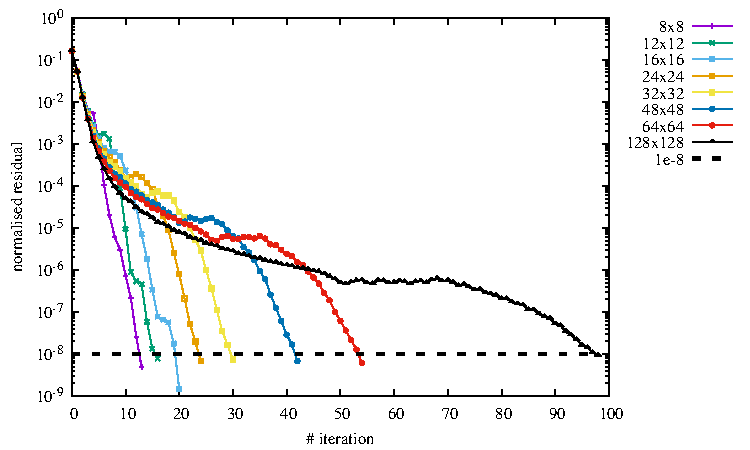
\includegraphics[width=10cm]{python_codes/fieldstone_15/results/residual.pdf}
\end{center}

\todo[inline]{build S and have python compute its smallest and largest eigenvalues as a function of resolution?}
